\documentclass[DIN,pagenumber=false,parskip=half,fromalign=left,fromphone=true,fromemail=true,fromurl=false,fromlogo=false,fromrule=false]{scrlttr2}
\usepackage[utf8]{inputenc}
%\usepackage{ngerman}
\usepackage[english]{babel}
\usepackage{units}
\usepackage{tabularx}
\usepackage{booktabs}
\usepackage{multirow}
\usepackage{xcolor}
\usepackage{graphicx}
\usepackage[right]{eurosym}
\usepackage{amsmath,amsfonts,amssymb}
\usepackage{braket}
\usepackage{graphicx}
%\RequirePackage{graphicx}

\setkomavar{fromname}{Dr. Elke Faßhauer}
\setkomavar{fromaddress}{Department of Chemistry\\University of Troms\o --- The Artic University of Norway\\9037 Tromsø\\Norway}
\setkomavar{fromphone}{+47 40382485}
\setkomavar{fromemail}{elke.fasshauer@uit.no}
\setkomavar{subject}{Revision of Out Article jp-2016-06665e}
\setkomavar{signature}{Dr. Elke Faßhauer (corresponding author)}


\begin{document}
\begin{letter}{To the Editor}
	
	\opening{Dear Editor,}


Our paper has been reviewed by two of your Referees,
who recommended it for the publication in the
New Journal of Physics subject to minor amendments.
We are thankful for the comments made by the Referees and
respond to them below. We additionally reply on two of the additional
format requests made by Ms. Maja Vujovic.

\textbf{Referee \#1} raised the following points:

\begin{enumerate}
 \item \emph{In general, I find the manuscript clearly written but unnecessary long. Some details and discussions can be avoided without weakening the presentation. Here are some examples:}
  \begin{enumerate}
   \item \emph{ICD is explained twice in the introduction (top of page 3 and
         3rd paragraph of page 3)}\\
				
				We have deleted the explanation of ICD in the 3rd paragraph of page 3.
				
   \item \emph{the sentence: The notion of ICD requires that the electronic orbitals … can be distinguished... make a distinction between ICD and Auger decay. does not bring important informations. Furthermore, using only a one-particle picture to define ICD may be misleading. For example, in molecular clusters ICD can be clearly identified after deep ionization (typically for binding energy above 20 eV) of one molecule. However, owing to the strong electronic correlation in this binding energy range the states cannot be described as ionization from a single orbital.}\\\vspace{0.3cm}\\
				The referee is correct, the statement does not bring new information. We have therefore deleted this section from the manuscript. That is also in accordance to the referees notion that the manuscript is too long. 
  
	\item \emph{Page 9: the sentence “These atoms do not necessarily need to form bonds...” just rephrases what is already explained earlier in the manuscript on ICD.}\vspace{0.3cm}\\
         The comment skips the important part of the argumentation, which is
         that the units/atoms do not need to be close. The comment about the
         bonding situation was made intentionally to clarify the difference
         between pairs and triples on the one hand and dimers and trimers on
         the other hand. We therefore do not change the sentence.

   \item \emph{Page 10: the definition of open and close channel is repeated. Explanations in page 9 and figure 1 are enough.}\vspace{0.3cm}\\
         The explanation on page 10 belongs to the explanation on page 9, which
         would not be understandable without half of the text. While the
         text formulates the general concept, the figure illustrates this concept
         on an example which is this manuscript's system under investigation.
         Since also the caption of the figure should be understandable without
         reading the text, we do not shorten the manuscript at this point.

   \item \emph{Page 13:
         the section “Cluster Structures” can be moved to Supporting information since only Table 2 is important to understand the results. Furthermore, it seems to me that the paragraph on previous study of the authors on large clusters does provide relevant informations on the reported results.}\vspace{0.3cm}\\
     The whole section consists of only four paragraphs in total and is rather short. The cluster structures are crucial for understanding the underlying theory and results. It is a very descriptive part of the manuscript and helps the reader to assess the different structures and classes under discussion. We therefore think that it will not improve the MS if the whole section is moved to the supplementary information. (note that a large part of this section is already there).

   \item \emph{Page:
         the section Outer valence spectra is very detailed and the reader may lose the main point of this section which is, as far as I understood, to evaluate experimentally the percentage of Xe in the clusters. All extra details can be avoided. Just to help the readers, this section could be renamed to highlight the goal of the section like for example “Xe content”.}\vspace{0.3cm}\\
				The referee is correct if one reads the article from a theoreticians point of view. However, the outer valence spectra of our clusters were not reported in this detail earlier nor were they ever discussed. We therefore think that this section holds very valuable information for the experimentalist which we do not want to hide in the supplementary section. To accommodate the referees suggestion we have included two sentences in the beginning of the section, summarizing the points that are most important for the theory part of the article: {\color{blue}{This section describes and discusses the outer valence spectra of the mixed Ar-Xe clusters. The main information we obtain from these spectra within the context of our theoretical considerations are
the single ionization potentials and
the relative Xe contents in the mixed cluster.}}
				
   \item \emph{Page:
         I think the section Inner valence spectra can be skipped without losing any relevant informations.}\vspace{0.3cm}\\
         Here we disagree with the referee. The presentation and discussion of the inner valence spectra is very relevant because they form the basis for our theoretical considerations. Additionally, they provide further direct insight into the structure of our clusters. An experimentally interested reader would surely miss the information provided here.

  \end{enumerate}

  \item \emph{Page 8:
        the authors write that “the intensities of the peaks are proportional to the probability decay as well as the decay width”. However, the probability and the width are simply related : Prob =  Width*time/hbar.}\\
				
        We included the relation between the decay probability and the decay
        width. However, the important information of this sentence is that
        the decay widths can be used to describe the intensities of the
        different peaks. Therefore, its proportionality is important. The
        sentence now reads:\\
        The latter is proportional to the
probability of the decay {\color{blue}{$P=\frac{\Gamma t}{\hbar}$}}
as well as the theoretically determinable
decay width $\Gamma=\frac{\hbar}{\tau}$,
which is inversely proportional to the lifetime $\tau$ of the decay process.

  \item \emph{Page 11:
        Eqs 6 and 7 the sums run over ALL pairs and ALL triples. In that case there should not be $N_{ICD,i}$ and $N_{ETMD,j}$ in the sums; otherwise those pairs and triples are counted several times.}\\
        It now reads:\\
        These are given by the sum over the decay widths of all 
        {\color{blue}{geometrically different}} pairs $i$ for the
        ICD and all {\color{blue}{geometrically different}} triples $j$
        for the ETMD(3),
        respectively, and over all channels $\beta$:

  \item \emph{Page 12:
        some symbols are not defined: $\Phi_{in}$, $\chi_\beta$, $H_f$
        for example.
        Since this part of theory has already been published, it can be shorten
        leaving just Eqs. 9 and 10.}\\
        This part of the theory has indeed been published already. However,
        the general formula for the decay width of electronic decay processes
        serves as the best starting point for the explanation since it is
        known by a wider community. For the same reason, equation 11 should
        be shown, as it connects the earlier formulation and the new more
        abstract formulation in equation 10. We therefore rephrased the
        paragraph to read:\\
        {\color{blue}{
        \begin{equation}
         \Gamma_{\beta}(E_{\rm res}) = 2\pi \left|
                                   \braket{\Phi_{\rm in}| \hat{V} |\chi_{\beta}}
                                   \right|^2,
        \end{equation}
%
where $\ket{\Phi_{\rm in}}$ and $\ket{\chi_{\beta}}$ are the initial and final
state, respectively and $\hat{V}$ is the interaction operator between these
two, can be approximated by its asymptotic behaviour.
For the ICD the approximation reads:}}
%
\begin{equation}
 \Gamma_{{\rm ICD},i,\beta} = (2J_{\rm in}+1)\, \frac{3c^4}{8\pi}\,
                        \sum\limits_{M_{in}'}
                        \left| \left(
                        \begin{array}{ccc}
                        J_A'  & 1        & J_A\\
                        -M_A' & M_A'-M_A & M_A
                        \end{array}\right) \right|^2
                        \frac{\sigma^{(X_E)}(\omega_{vp,\beta})}
                        {R_i^6 \, \omega_{vp,\beta}^4 \tau_{in,\beta}},
\end{equation}                                                 
%
where $J_A$, $J_A'$ and $M_A$, $M_A'$ denote the total angular momentum of the
initially ionized atom (which is the same as the electron donor atom) in the 
initial and final state, respectively,
{\color{blue}{which otherwise depends on
intrinsic atomic properties
which can be determined experimentally, like the ionization
cross sections
$\sigma^{(X_E)}(\omega_{vp,\beta})$, radiative lifetimes of the initially
ionized state $\tau_{in,\beta}$ and the excess energy transferred to the
emitting atom (the energy of the virtual photon) $\omega_{vp,\beta}$.

For the ETMD(3) the approximation reads}}
%
\begin{align}                                                  
 \Gamma_{{\rm ETMD},j,\beta} =& \frac{c}{\pi} \sum\limits_{m,M_{in,D'}}      
                        \frac{\Theta_{m,k}(\alpha_j) \sigma^{(X_E)}(\omega_{vp,\beta})
                              \left| <\tilde{D}_{m,j,\beta}(M_{in,D'})>\right|^2}
                         {R_j^6 \omega_{vp,\beta}}\\           
               =& \frac{c}{\pi R_j^6}                          
               \sum\limits_{M_{in,D'}}                         
               \left( \left| <\tilde{D}_{x,j,\beta} (M_{in,D'}) > \right|^2  
                 (2+ \sin^2\alpha_j)                           
               + \left| <\tilde{D}_{z,j,\beta} (M_{in,D'}) > \right|^2       
                 (1+\cos^2\alpha_j) \right) \nonumber \\       
           & \times\, \frac{c\sigma^{(X_E)}(\omega_{vp,\beta})}{\omega_{vp,\beta}}
\end{align}                                                    
%                                                              
{\color{blue}{
where $\tilde{D}_{m,j,\beta}$ are calculated transition dipole moments and}}
$\Theta_{m}(\alpha_j)$ is a function depending on the angle $\alpha_j$       
of the triple and the direction of the dipole                  
transition moment $m$ ...

  \item \emph{Page 12:
        ionization cross-sections, radiative lifetimes,... are not EXPERIMENTAL properties of atoms, they are intrinsic properties of atoms that can be experimentally measured.}\\
        Agreed. The sentence now reads:\\
        ... on {\color{blue}{intrinsic atomic properties
        which can be determined experimentally}}, like the ionization
        cross sections
        $\sigma^{(X_E)}(\omega_{vp,\beta})$, radiative lifetimes of the initially
        ionized state $\tau_{in,\beta}$ ...
 
  \item \emph{As far as I understand Figs 4-8 report Widths with respect to Electron energy and are thus not strictly speaking electron emission spectra. The authors should really compute the spectra. Furthermore, the lines which I guess are some convolution of the bars are not defined. And more importantly, how these “spectra” were normalized is not clear: in the cluster with 55 Ar atoms the central and inner layer of atoms can undergo ICD. A more intense band compared to 13 atoms is therefore expected. More explanations are needed.}\vspace{0.3cm}\\
        The first part of the reviewer's comment is confusing. We have clearly
        explained the direct proportionality between the decay width and
        the probability of the decay for a given initial and a given final state,
        which is also related to a specific kinetic energy of the emitted
        electron. This gives a stick spectrum within the limitations
        of the model as explained in the theory section. The convoluted stick
        spectrum then gives the estimated spectrum
        (for details see the adjustments made for
        comment to reviewer \# 2 point 2).\\
        In terms of the normalization we agree with the reviewer that this part
        was not explicitly described and we therefore added the following
        paragraph to the theory section:\\
        {\color{blue}{The decay width for the total system is in the end
        normalized to the decay width
        per initially ionized atom since we are interested in the events
        after one ionization which could be located at any of the atoms of
        the corresponding atom
        type. We thereby yield an averaged decay width for the cluster structure.
        This step allows the comparison of the total average decay widths
        between cluster structures of different size and composition.}}
        \vspace{0.3cm}\\
        This means, that in the 13 and 55 atoms argon clusters with one
        additional xenon atom
        located on one of its surfaces, there are 13 or 55 potentially
        initially ionized atoms. Inspecting Figure 4, lower panel, it is
        evident, that the number of pairs for which all decay channels are
        closed is similar for the 14 and the 56 atom cluster. However,
        the distribution of pairs with open decay channels is significantly
        different. The 14 atom cluster has only a few more pairs which are
        characterized by comparably small distances. Therefore, each of these
        pairs will have a significant decay width. In case of the 56 atoms
        cluster there are many pairs with open channels characterized by many
        different distances and especially much larger distances than in the
        14 atoms cluster. Therefore, the average decay width is smaller in the
        56 atoms cluster than in the 14 atoms cluster.
        The reviewers intuition would be correct if the atom types of argon
        and xenon atoms were interchanged.

  \item \emph{Page 18:
        it is stated that the decay width decreases like R-6 but in page 20 it decreases exponentially.}\\
        The reason is that it discusses different interatomic distances being
        the energy transfer distance $R$ ($R^{-6}$) and the electron
        transfer distance $Q$ ($e^{-Q}$) which can both be found in previous and
        coming papers about ETMD(3) (J. Chem. Phys. \textbf{138}, 014305 (2013).
        and Fasshauer \emph{et al.} Mol. Phys. (2016), submitted.):
\begin{center}
 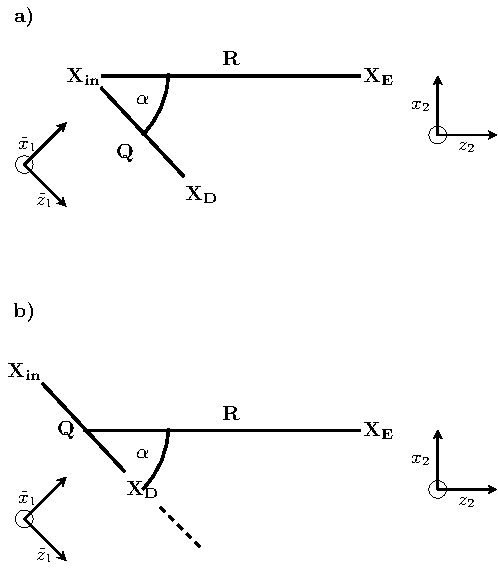
\includegraphics[width=6cm]{../pics/coord_systems.pdf}
\end{center}
        Both on page 18 and 20, these distances are very clearly characterized
        in terms involved atom types or groups and which process is ongoing.
        To further clarify the matter, the sentences on page 18 now read:\\
        Two aspects have to be taken into account: an energy shift of the peaks
        due to different charge distances {\color{blue}{$d$}} in the
        final state (i.e. the interatomic Xe-Xe
        distance) and the decrease of the decay width with $R^{-6}$,
        $R$ being the distance between the electron transfer unit and the xenon
        atom ionized in the final state.
        The larger the distance between the xenon atoms, the higher are the
        energies of the secondary electrons{\color{blue}{. For the case of xenon
        atoms on argon surfaces this at the same time means a larger distance
        between the Ar-Xe pair involved in the electron transfer and the
        electron emitting xenon atom. Hence, the decay widths are smaller.}}
        Therefore, a
        significant contribution from ETMD(3) compared to ICD is only
        seen if the two xenon atoms reside on two adjacent
        surfaces. 

  \item \emph{Page 29:
        the efficiency of ICD is found below unity for clusters having few Xe atoms. I guess this is because in these clusters ICD and ETMD are closed for some Argon atoms which are anyway ionized. Maybe a statistical model may explain it. The theory could also help since it should be easy to determine the efficiency for all clusters considered in this study.}\vspace{0.3cm}\\
        This is a good point from the referee. We have included a short discussion of the possible explanations of this effect at the respective place: {\color{blue}{We found an Ar 3s autoionization efficiency which is compatible with unity, within the accuracy of our experiment, for all clusters except those with the lowest Xe content (Xe$_{\rm cl}$ approx. 10-12\,\%).
For the latter, also a decrease of the efficiency with decreasing cluster size is seen. 
Two main reasons can be identified that may cause a decrease in autoionization efficiency. 
Firstly, in small clusters with a low Xe content, for some Ar atoms no Xe partners allowing either ICD or ETMD might be available.
A simple example are clusters containing just a single Xe atom.
This mechanism would gain in importance for cluster ensembles with small $\langle N\rangle$.
Secondly, if only Xe partners at very large distances are available, ICD might be outpaced by other decay processes, most importantly fluorescence.
}}


\end{enumerate}

\textbf{Referee \#2} raised the following points:

\begin{enumerate}
 \item \emph{ETMD(3) should be explained in the introduction by a sentence or two to aid the reader (at the moment, it is first explained in the theory section).
}\vspace{0.3cm}\\
       It was indeed explained already but in wording specific to
       experimentalists. We therefore changed the last paragraph on page 3 to:\\
       Soon after, related autoionization processes were discovered
       {\color{blue}{in which the initial vacancy is filled by an electron from a neighbouring unit. These were termed `Electron Transfer Mediated Decay'
(ETMD)$^{9–12}$. If the excess energy is transferred to a third unit which is subsequently ionized, the process is called ETMD(3), if the electron donor is ionized once more the process is called ETMD(2) and if the excess energy is used to ionize the initially ionized unit the process is called `exchange ICD'$^{13,14}.$}}

 \item \emph{The authors mention that the ‘nuclear dynamics may play an important role’ but that they have been neglected in the calculations. While I understand that it is not feasible in such large systems the authors should at least briefly discuss the possible effect of nuclear dynamics e.g. peak shifts, broadening, ICD vs. ETMD, etc. }\vspace{0.3cm}\\
       We added two paragraphs at the end of the theoretical results section
       discussing the possible effects of nuclear dynamics:\\
       {\color{blue}{All these results neglect the effect of nuclear dynamics, which might affect the spectra. Possible reasons are distance dependent channel closings and openings, a different distribution of interatomic distances due to vibrations and their different impact on the ICD and the ETMD(3). E.g., for the ICD in the neon dimer, the treatment of nuclear dynamics increases the decay width by approximately a factor 2.$^{57}$ However, the atomic displacement can be expected to be far less severe in clusters than in dimers or trimers. Additionally, the
elongation of one interatomic distance in a cluster automatically results in the shortening of a different interatomic distance, which will reduce the overall effect. Therefore, there will be a broader spectrum of final state charge
distances $d$ resulting in a broadening of the peak. This was taken into
account by folding the stick spectrum with Gaussians with a width of 300 meV and 600 meV for the ICD and ETMD(3), respectively. While the width of the ICD peaks was estimated from the potential energy surface of the ArXe dimer, the situation is more complex in case of the ETMD(3) with three degrees of freedom involved. It was therefore guessed to be twice the width of the ICD peak.

The channel closing due to shortening of the interatomic distance is not
relevant for the ETMD(3) process in the ArXe clusters treated in this work,
because this would require unnaturally short interatomic distances.
However, for the ICD it might result in a lower number of pairs with open
decay channels and hence a decrease of the decay width. 
Since the peaks in the convoluted spectrum 
contain contributions from several atom pairs at different distances, 
this would result
in a small peak shift to higher energies of the combined peak at lowest energy.
For a more detailed discussion of nuclear dynamics for the ICD in dimers vs.
clusters see Ref. 58.
}}


 \item \emph{The spin-orbit splitting of the Ar 3p$^{-1}$ state is briefly mentioned in Table 3 in the experimental section but it also stated that the a single value of the binding energy of Ar 3p equal to 15.3 eV is used for all of the simulations. The authors should explain the motivation for this choice in the theory section.}

The reason is that the clusters do not show spin-orbit splitting as opposed to the monomer. To make this more clear we have included a sentence in the "outer valence" section: {\color{blue}{ A distinction between the Ar 3p $_{1/2}$ and the Ar 3p $_{3/2}$ derived cluster bands can therefore not be made.}}

 \item \emph{Page 13:
       The authors should justify the use of the ‘unified force field’ method for the calculation f the cluster structure (p13).}
       We added a sentence to justify our choice:\\
       After that, the cluster structures were optimized using the unified
       force field implemented in the Avogadro programme
       (version 1.1.0)$^{51,52}$ to give local minimum structures.
       {\color{blue}{ The method
       was chosen due to its low computational cost, the possibility to find
       the next local minimum structure based on the chosen starting point
       and the necessary effort to produce reliable results with density
       functional theory (DFT) for v. d. Waals interactions since in
       this work we discuss structural trends and not absolute structures.}}

 \item \emph{Page 12:
       On page 12 last line there is to Tables II and III. I have not been able to locate these. The reference should be clarified.}\\
       The sentence has been changed to:\\
       In this work we evaluate the secondary energies and decay widths with
       the programme HARDRoC$^{20,49}$ using the experimental ionization energies
       of Table 3 and data from the literature given in Tables II and III
       {\color{blue}{of Ref. 34.}}\\
       The following sentence was removed.

 \item \emph{Page 20,21:
       it is not clear what structure of the larger clusters with 3871 atoms is used in the simulation. The authors mention icosahedral and cuboctahedral but no further details are given, e.g. Ar-Xe distance, Ar-Ar distance, etc.}\\
       The details were added to the Cluster Structures section. The last
       sentences now read:\\
       Furthermore, for comparison with the largest measured ArXe clusters,
       we constructed also larger core-shell structures (Table 2, \#4 – 5).
       {\color{blue}{These were idealized icosahedral and cuboctahedral
       structures based on the v. d. Waals radii of argon and xenon
       $r_{Ar} =$\unit[1.88]{\AA}$^{54}$
       and $r_{Xe} =$\unit[2.16]{\AA}$^{55}$.}}

 \item \emph{In fig. 9(a) it is specified in the text that  Ar $<N>$ =190 for the black trace but as far as I can tell no value is given for the other spectrum on the same graph.}

	We have clarified the information in the figure caption and additionally refer to the respective table.

 \item \emph{It is not clear what the dotted lines in Figure 10 are?}

 We have clarified the information in the figure caption by including the sentence: {\color{blue}{The dotted line shows the unscaled spectrum in this region.}}

 \item \emph{The colour schemes of some of the figures lead to confusion when printed in grayscale. Some effort could be made to resolve this.}\vspace{0.3cm}\\
       The reviewer does not specify which figures are affected by this.
       We therefore assume a reference to figures 4-8. In these, the
       information density is very high, especially within the stick spectrum.
       Due to this, overlapping dotted or dashed lines would not be
       decipherable and only confuse the reader not only on a grayscale print
       but also a coloured print. Since the majority of scientific journals
       at least have the pdf version available as well, we therefore leave
       the colour choice, which was made to allow readability by
       colour blind people as well.

\end{enumerate}

We also applied almost all requested changes to the format of the manuscript.
Request number 4 (remove unpublished results from References) asks for
published and sonn-to-be published material. Since the manuscript in
questions was submitted a month ago and was an invited contribution
for special issue to be published in October at the latest.
We expect this manuscript
will become published then. We also interpret this timeframe as soon
and therefore leave the Reference in the list.

For point 6 see Reviewer 2 point 5.



        \closing{Sincerely yours,}
	\end{letter}

\end{document}
